% !TEX program = lualatex
% !TEX program = lualatex
%
% Poster v3: Bayes-assisted anytime-valid t-tests for Gaussian means
%            with unknown variance.
% Revised to follow supervisor storyline:
%   * t-tests motivation (no prior info -> with prior info)
%   * explicit "why classical Ville loses all power under mismatch"
%   * removal of CS references
%   * composite-prior framing of unknown-variance extension
%   * trichotomy block as prose (no big tikz)
%   * simulation legend in caption

\documentclass[final]{beamer}

\usepackage[T1]{fontenc}
\usepackage{lmodern}
\usepackage[orientation=landscape,size=a0,scale=1.0]{beamerposter}
\usetheme{gemini}
\usecolortheme{oxford}
\usepackage{graphicx}
\usepackage{booktabs}
\usepackage{tikz}
\usepackage{pgfplots}
\usepackage{natbib}
\usepackage[dvipsnames]{xcolor}
\usepackage{amsmath,amssymb,amsfonts,mathtools,bm}
%\usepackage{xcolor}
\pgfplotsset{compat=1.14}
\setbeamercolor{alerted text}{fg=oxfordblue}
\definecolor{DeepGreen}{RGB}{0,120,0}
% ====================
% Math macros (from the report)
% ====================
\newcommand{\E}{\mathbb{E}}
\newcommand{\Prob}{\mathbb{P}}
\newcommand{\dd}{\,\mathrm{d}}
\newcommand{\Leb}{\mathrm{Leb}}
\newcommand{\Lap}{\mathrm{Lap}}
\newcommand{\thetahat}{\widehat{\theta}_n}

% ====================
% Lengths
% ====================
\newlength{\sepwidth}
\newlength{\colwidth}
\setlength{\sepwidth}{0.025\paperwidth}
\setlength{\colwidth}{0.3\paperwidth}

\newcommand{\separatorcolumn}{\begin{column}{\sepwidth}\end{column}}

% ====================
% Title
% ====================
\title{Bayes-assisted anytime-valid \texorpdfstring{$t$}{t}-tests for Gaussian means with unknown variance}
\author{Debolina Paul \and Patrick Rebeschini \and Fran\c{c}ois Caron}
\institute[shortinst]{Department of Statistics, University of Oxford}

\footercontent{%
  \href{mailto:debolina.paul@stats.ox.ac.uk}{debolina.paul@stats.ox.ac.uk}%
}

\logoright{
\includegraphics[height=10cm]{ox_logo.pdf}}

\begin{document}
\begin{frame}[t]
\begin{columns}[t]
\separatorcolumn

% ============================================================
% COLUMN 1 -- Motivation, Setup (with "why eV"), Lebesgue closed form
% ============================================================
\begin{column}{\colwidth}

  \begin{block}{Motivation}
  % Anytime-valid $t$-tests for unknown-variance Gaussians arise various real-world problems such as in clinical trials, A/B testing, sequential quality monitoring etc. The no-prior framework is well understood \cite{Lai1976,PerezOrtiz2024,Wang2025}. With prior information, mixture martingales calibrated by Ville's inequality yield anytime-valid Bayes factors \cite{Rouder2009}, \alert{but any proper informative prior loses all power under prior--data mismatch},
$t$-tests are widely used in clinical trials, A/B testing, quality monitoring etc., providing a standard method for inference on Gaussian means when the variance is unknown. In many such applications, however, data are collected sequentially, which has motivated the development of anytime-valid extensions.

\textbf{Existing approaches:}
%\vspace{-0.4cm}
\begin{itemize}
  \setlength\itemsep{0.08cm}
  \item \textbf{No prior information} \cite{Lai1976,PerezOrtiz2024,Wang2025}: scale-invariant likelihood ratio calibrated by Ville's inequality, but \textcolor{red}{unable to exploit prior knowledge.}
  \item \textbf{With prior information} \cite{Rouder2009, gronau2020informed}: informative-prior Bayes factor, made anytime-valid as a mixture martingale via Ville's inequality, but \textcolor{red}{any proper informative prior loses all power under prior-data mismatch.}
\end{itemize}

%\alert{Any proper informative prior loses all power under prior--data mismatch:} 
  %\vspace{0.2cm}
  \begin{center}
  \begin{tikzpicture}[scale=2, every node/.style={font=\footnotesize}]
    % --- axis and true effect ---
    \draw[->, thick] (-3, 0) -- (9, 0) node[below right] {$\theta$};
    \draw[blue!80!black, dashed, very thick] (0.5, 0) -- (0.5, 2.5);
    \node[blue!80!black, anchor=south west] at (0.55, 2.5) {$\theta^\star$};

    % --- likelihood concentrated at theta* ---
    \draw[thick, blue, smooth, samples=80, domain=-1:2]
      plot (\x, {2.2 * exp(-(\x - 0.5)^2 * 5)});
    \node[blue, anchor=east] at (-0.6, 1.7) {likelihood};

    % --- aligned prior ---
    \draw[thick, green!50!black, smooth, samples=80, domain=-3:4]
      plot (\x, {1.3 / (1 + 0.8*(\x)^2)});
    \node[green!50!black, anchor=east] at (-1.15, 0.7) {$\Pi_{m=0}$};

    % --- misaligned prior ---
    \draw[thick, red!75!black, smooth, samples=80, domain=2.5:9]
      plot (\x, {1.3 / (1 + 0.8*(\x - 6)^2)});
    \node[red!75!black, anchor=west] at (7.5, 0.7) {$\Pi_{m \gg 0}$};

    % --- outcome labels ---
    \node[align=center, green!50!black] at (0.5, -0.65)
      {\textbf{agreement} \\ $M_n^{\Pi} \nearrow$ rejects};
    \node[align=center, red!75!black] at (6, -0.65)
      {\textbf{mismatch} \\ $M_n^{\Pi}\to 0$, never rejects};
  \end{tikzpicture}
  \end{center}
  \vspace{0.15cm}

  As $|m|\to\infty$, $M_n^{\Pi_m}\to 0$ so $P_n^V=\min \left\{\frac{1}{M_n^{\Pi_m}}, 1\right\} \to 1$, the procedure simply never rejects.
  \vspace{0.1cm}
%   \textbf{Our contribution.} \cite{Cortinovis2025} addressed this for a simple null for i.i.d. Gaussian data where the variance known. We extend from known to \alert{unknown variance}, where the prior is composite on $(\theta,\sigma)$, via the \alert{extended Ville inequality} \cite{wang2025extended}: Let \((X_n)_{n\geq 1}\) be an extended nonnegative supermartingale.
% For any \(c>0\),
% \[
%    \Prob\left(\sup_{n\geq 1} X_n\geq c\right)\;\leq\;
%    \E\!\bigl[\min(X_1/c,\,1)\bigr] = g(c).
% \]
  
%   Then, for any $\sigma$-finite (proper \emph{or} improper) $\Pi$,
%   \[
%     P_n \;=\; g_\Pi\!\bigl(M_n^{\Pi}\bigr), \qquad
%     g_\Pi(c) \;=\; \E_{H_0}\!\bigl[\min(M_2^{\Pi}/c,\,1)\bigr]
%   \]
%   is a valid $p$-process. The resulting informative $p$-processes gain power under agreement and \alert{revert to the Lebesgue baseline} under conflict.
\textbf{Our contribution.} \cite{Cortinovis2025} addressed prior-data conflict in the known variance Gaussian setting, but real applications almost always involve \alert{unknown variance}. We extend the framework to this case, where $\sigma$ enters as a nuisance parameter and the prior is composite on $(\theta,\sigma)$. The proposed method gain power under prior-data agreement and \alert{revert to the non-informative Lebesgue baseline} under arbitrary conflict.


%for a simple null with known variance. We extend to the practically central case of \alert{unknown variance}, where $\sigma$ enters as a nuisance parameter and the prior is composite on $(\theta,\sigma)$ without losing power even in data-prior conflict. %The construction yields informative $p$-processes that gain power under prior--data agreement and \alert{revert to the non-informative Lebesgue baseline} under arbitrary conflict --- recovering an anytime-valid analogue of Lai's classical $t$-statistic at no worst-case efficiency cost.
\end{block}
%\vspace{-0.1cm}
  \begin{block}{Setup}
$Y_1,Y_2,\ldots\stackrel{\mathrm{iid}}{\sim}\mathcal N(\mu,\sigma^2)$, both parameters unknown; standardised effect $\theta^\star=\mu/\sigma$. Test
    \[
      H_0\colon\theta^\star=0 \quad\text{vs}\quad H_1\colon\theta^\star\neq 0.
    \]
    A \alert{$p$-process} $(P_n)_{n\ge 2}$ satisfies $\Prob_{H_0}(\exists n\colon P_n\le\alpha)\le\alpha$, so rejecting at the first crossing is valid under every data-dependent stopping rule.
    %\vspace{-0.1cm}
    
    \textbf{Scale-invariant likelihood ratio.} On the filtration $\mathcal F_n=\sigma(Y_i/|Y_1|)$, after integrating out $\sigma$ against its Haar measure,
    %\vspace{-0.1cm}
    \[
      L_n(y_{1:n};0,\theta) \;=\; \frac{h_{\theta,n}(y_{1:n})}{h_{0,n}(y_{1:n})},\]
      \[
      h_{\theta,n}\;=\;e^{-n\theta^{2}/2}\,A_n(\theta\,u_n),
    \]
    %\vspace{-0.1cm}
    with $A_n(z)=\E[e^{zX}]$, $X\sim\chi_n$, and maximal invariant
    \[
      u_n \;=\; \frac{\sum_{i=1}^n y_i}{\sqrt{\sum_{i=1}^n y_i^{2}}}
           \;=\; \frac{n\,\thetahat}{\sqrt{(n-1)+n\,\thetahat^{\,2}}}\;\in\;[-\sqrt n,\sqrt n].
    \]

    %\vspace{-0.1cm}
    \textbf{Mixture martingale.} For $\sigma$-finite $\Pi$ on $\mathbb R$,
    \[
      M_n^{\Pi}(y_{1:n}) \;=\; \int_{\mathbb R} L_n(y_{1:n};0,\theta)\,\Pi(\dd\theta).
    \]
    %\vspace{-0.2cm}
    \textbf{Why classical Ville is not enough.}
    %\vspace{-0.2cm}
\begin{itemize}
  \setlength\itemsep{0.08cm}
  \item \textbf{Proper $\Pi$:} $M_n^\Pi$ is a non-negative martingale and Ville gives $P_n^{V,\Pi}(y_{1:n})=\frac{1}{M_n^\Pi(y_{1:n})}$. But \alert{every proper prior is fragile}: power $\to 0$ as $|m|\to\infty$.
  \item \textbf{Lebesgue baseline:} restores power but is \emph{improper}; $\E_{H_0}[M_n^{\Leb}]=\infty$, so the classical bound $1/c$ no longer applies.
\end{itemize}
%\vspace{-0.1cm}
% The \alert{extended Ville inequality} \cite{wang2025extended} circumvents both:
% \[
%    P_n^{E,\Pi}(y_{1:n})=g_\Pi\!\bigl(M_n^\Pi(y_{1:n})\bigr),
%    \qquad
%    g_\Pi(c)=\E_{0}\!\left[\min\!\left(\tfrac{M_2^\Pi(Y_{1:2})}{c},\,1\right)\right],
% \]
% a valid $p$-process for proper \emph{and} improper $\Pi$. This is what lets an informative $\Pi_m$ revert to the Lebesgue baseline under conflict while \alert{always} delivering a valid $p$-process — unlike a Bayes factor, whose interpretation breaks under mismatch.
%     \textbf{Why classical Ville is not enough.} For proper $\Pi$, $M_n^\Pi$ is a non-negative martingale and Ville gives $P_n^{V,\Pi}(y_{1:n})=\frac{1}{M_n^\Pi(y_{1:n})}$. But \alert{every proper prior is fragile under conflict}: power $\to 0$ as $|m|\to\infty$. Restoring power requires the (improper) Lebesgue baseline, but then $\E_{H_0}[M_n^{\Leb}]=\infty$ and the classical Ville bound $1/c$ no longer applies.

%     %\vspace{0.05cm}
%     The \alert{extended Ville inequality} (Wang \& Ramdas 2025b) circumvents this,
%     \[
%      P_n^{E,\Pi}(y_{1:n})=g_\Pi(M_n^\Pi(y_{1:n})),
% \qquad
% g_\Pi(c)=\E_{0}\!\left[\min\!\left(\frac{M_2^\Pi(Y_{1:2})}{c},1\right)\right],
%     \]
%     is a valid $p$-process for proper \emph{and} improper $\Pi$. This is the property that lets an informative $\Pi_m$ revert to the Lebesgue baseline under conflict, while \emph{always} delivering a valid $p$-process, unlike a Bayes factor whose interpretation breaks under mismatch.
  \end{block}
\end{column}

\separatorcolumn

% ============================================================
% COLUMN 2 -- Trichotomy (prose) + exponential tilt + Laplace directional
% ============================================================
\begin{column}{\colwidth}
\begin{alertblock}{Proposal: extended Ville calibration}
\textbf{Key tool.} For any extended non-negative supermartingale $(X_n)_{n\ge 1}$, the \alert{extended Ville inequality} \cite{wang2025extended},

\[ \Prob_{H_0}\!\left(\sup_{n\ge 1} X_n \ge c\right) \le \E_{H_0}\!\left[\min\!\left(\frac{X_1}{c},1\right)\right] =: g(c). \] 
Moreover, \[ g(c) \le \min(1/c,1), \] with equality only in the degenerate case. Thus extended Ville calibration is at least as sharp as Ville's bound, and remains valid when Ville's inequality is not applicable.
  % We sidestep both failure modes by replacing Ville's inequality with the \alert{extended Ville inequality} \cite{wang2025extended}, which holds for an arbitrary extended non-negative supermartingale $(X_n)_{n\ge 1}$:
  % \[
  %    \Prob_{H_0}\!\Bigl(\sup_{n\ge 1} X_n\ge c\Bigr) \;\le\; \E_{H_0}\!\bigl[\min(X_1/c,\,1)\bigr] \;=:\; g(c).
  % \]
  % Crucially, $g(c)\le\min(1/c,1)$, with equality only when $X_1$ is degenerate --- so the extended-Ville bound is \alert{uniformly at least as sharp} as Ville's $1/c$, and \emph{tight even when $X_1$ has infinite mean}, the regime where Ville breaks.

  \vspace{0.10cm}
  \textbf{Application to mixture martingales.} For any $\sigma$-finite mixing measure $\Pi$, proper or improper, define \[ P_n^{E,\Pi}(y_{1:n}) = g_\Pi\!\left(M_n^\Pi(y_{1:n})\right), \] where \[ g_\Pi(c) = \E_{H_0}\!\left[ \min\!\left( \frac{M_2^\Pi(Y_{1:2})}{c},1 \right) \right]. \]
  % \textbf{Applied to mixture martingales.} For any $\sigma$-finite (proper \emph{or} improper) $\Pi$, setting $X_n = M_n^{\Pi}$ gives the valid $p$-process
  % \[
  %    P_n^{E,\Pi}(y_{1:n}) \;=\; g_\Pi\!\bigl(M_n^{\Pi}(y_{1:n})\bigr), \qquad
  %    g_\Pi(c) \;=\; \E_{H_0}\!\Bigl[\min\!\Bigl(\tfrac{M_2^{\Pi}(Y_{1:2})}{c},\,1\Bigr)\Bigr].
  % \]
  % \alert{Validity holds for any $\Pi$ --- proper or improper, well-specified or misaligned}: there is no regime in which the $p$-process becomes meaningless, in contrast to a Bayes factor whose interpretation breaks under mismatch.

  \vspace{0.10cm}
  \textbf{Consequence.} The resulting process is a valid $p$-process for any $\Pi$: \[ \Pi \text{ may be proper, improper, well-specified, or misaligned.} \] Hence calibration does not rely on a Bayes-factor interpretation. 
  
  \vspace{0.08cm} 
  \textbf{Limits.} This makes the non-informative limit $\Pi=\Pi_{\Leb}$ usable, while the informative limit $\Pi=\Pi_m$ interpolates automatically between the two regimes. 
  % The non-informative limit $\Pi = \Pi_{\Leb}$ is now usable; the informative limit $\Pi = \Pi_m$ with a polynomial-tail $\pi$ will be shown (\S\textbf{Recovery}) to interpolate between the two automatically.
\end{alertblock}

\begin{block}{Closed form: Lebesgue prior recovers the scale-invariant \texorpdfstring{$t$}{t}-statistic}
    \textbf{Theorem 1.} Under $\Pi_{\Leb}(\dd\theta)=\dd\theta$, for $n\ge 2$ and $|u_n|<\sqrt n$,
    {\large
    \[
      M_n^{\Leb}(u_n) \;=\; \sqrt{\tfrac{2\pi}{n}}\Bigl(1-\tfrac{u_n^{2}}{n}\Bigr)^{\!-n/2} \;=\; \sqrt{\tfrac{2\pi}{n}}\Bigl(1+\tfrac{n\thetahat^{\,2}}{n-1}\Bigr)^{\!n/2}.
    \]}
    Up to the multiplicative constant, this is the scale-invariant $t$-statistic of \cite{Lai1976}.
    %, here promoted to an anytime-valid procedure via the extended Ville calibration $g_{\Leb}$.
    
    \vspace{0.1cm}
    \textbf{Theorem 2 (closed-form calibration).} With $B\sim\mathrm{Beta}(1/2,1/2)$, $M_2^{\Leb}=\sqrt\pi/B$, and
    \[
      g_{\Leb}(c) \;=\; \begin{cases}
        1, & 0<c\le\sqrt\pi,\\[2pt]
        \dfrac{2}{\pi}\!\left[\arcsin\!\sqrt{\tfrac{\sqrt\pi}{c}}+\sqrt{\tfrac{\sqrt\pi}{c}\bigl(1-\tfrac{\sqrt\pi}{c}\bigr)}\right], & c>\sqrt\pi,
      \end{cases}
    \]
    continuous, strictly decreasing on $[\sqrt\pi,\infty)$, one-to-one onto $(0,1]$.
  \end{block}



  % \begin{block}{Trichotomy of prior tails}
  %   For a prior $\Pi_m(\dd\theta)=\pi(\theta-m)\dd\theta$ shifted to $m$, the limiting behaviour of the rescaled mixture $M_{n,m}^{\Pi}(u_n)/a_m$ ($a_m$ a tail-rate of $\pi$) as $|m|\to\infty$ is governed by the prior's tail decay \emph{relative to the Gaussian envelope} $e^{-n\theta^{2}/2}$ of the likelihood:

  %   \vspace{0.20cm}

  %   \textcolor{green!50!black}{$\bullet$ \textbf{Polynomial}}, $\pi(\theta)\asymp |\theta|^{-\beta}$, $\beta>1$ (Cauchy, Student-$t_\nu$, horseshoe).\\[0.1cm]
  %   \hspace*{0.6cm} $M_{n,m}^{\Pi}/a_m\to M_n^{\Leb}$: the extended-Ville $p$-process \alert{reverts to the Lebesgue baseline} (Theorem 6).

  %   \vspace{0.18cm}
  %   \textcolor{orange!75!black}{$\bullet$ \textbf{Exponential}}, $\pi(\theta)\propto e^{-|\theta|/r}$ (Laplace).\\[0.1cm]
  %   \hspace*{0.6cm} Borderline case: $M_{n,m}/a_m^{\Lap}\to I^{\pm}(u_n)$, a non-trivial directional limit with residual rate $1/r$ (Theorem 4).

  %   \vspace{0.18cm}
  %   \textcolor{red!60!black}{$\bullet$ \textbf{Sub-Gaussian}}, $\pi(\theta)\lesssim e^{-\theta^{2}/(2\tau^{2})}$.\\[0.1cm]
  %   \hspace*{0.6cm} $M_{n,m}^{\Pi}\to 0$ super-exponentially: the procedure \alert{cannot reject regardless of the data} (Theorem 8).

  %   \vspace{0.20cm}
  %   \textbf{Polynomial-tail priors are the unique class with bounded influence and full anytime-validity under arbitrary conflict.} They thus combine the informative-prior efficiency of Rouder et al.\ (2009) with the robustness of an improper baseline.
  % \end{block}

  % \begin{block}{Closed form: one-sided exponential tilt}
  %   For $\kappa\in\mathbb R$ and location $m\in\mathbb R$, define the $\sigma$-finite composite prior
  %   \[
  %     \pi_\kappa(\theta,\sigma)\,\dd\theta\,\dd\sigma \;=\; \tfrac{1}{\sqrt{2\pi}\,\sigma}\,e^{-\kappa(\theta-m)}\dd\theta\,\dd\sigma,
  %   \]
  %   combining the right-Haar measure on $\sigma$ with a one-sided exponential tilt on $\theta$. Writing $T_n=\sum y_i^{2}$:

  %   \vspace{0.05cm}
  %   \textbf{Theorem 3.} For every $n\ge 2$ and $u_n\in(-\sqrt n,\sqrt n)$,
  %   \[
  %     M_n^{(\kappa)}(y_{1:n}) \;=\; \frac{(n-1)!}{(2\pi)^{n/2}\sqrt n}\!\left(\frac{T_n(n-u_n^{2})}{n}\right)^{\!-n/2}\! e^{\Lambda_n(\kappa,u_n)}\, D_{-n}\!\bigl(z_n(\kappa,u_n)\bigr),
  %   \]
  %   where $D_{-n}$ is the parabolic cylinder function and
  %   \[
  %     z_n(\kappa,u_n) = \frac{\kappa\,u_n}{\sqrt{n(n-u_n^{2})}},\qquad
  %     \Lambda_n(\kappa,u_n) = \kappa m + \frac{\kappa^{2}}{2n} + \frac{\kappa^{2} u_n^{2}}{4n(n-u_n^{2})}.
  %   \]
  %   At $\kappa=0$ this reduces to $M_n^{\Leb}$ via Legendre duplication and $D_{-n}(0)=\sqrt\pi\,2^{-n/2}/\Gamma((n+1)/2)$.
  % \end{block}

  % \begin{alertblock}{Directional limits of the symmetric Laplace mixture}
  %   For $\pi_{\Lap;m,r}(\theta)=(2r)^{-1}e^{-|\theta-m|/r}$ the mixture $M_{n,m}$ admits no closed form. After rescaling by $a_m^{\Lap}(r)=(2r)^{-1}e^{-|m|/r}$:

  %   \vspace{0.05cm}
  %   \textbf{Theorem 4.} Both directional limits exist; with $\kappa=1/r$,
  %   \[
  %     \lim_{m\to+\infty}\frac{M_{n,m}(u_n)}{a_m^{\Lap}(r)} = I^+(u_n), \qquad
  %     \lim_{m\to-\infty}\frac{M_{n,m}(u_n)}{a_m^{\Lap}(r)} = I^-(u_n),
  %   \]
  %   each coinciding with the one-sided exponential tilt of Theorem 3 at zero location, with opposite signed rates, and
  %   \[
  %     \frac{I^+(u_n)}{I^-(u_n)} \;=\; \frac{D_{-n}\!\bigl(-z_n(\kappa,u_n)\bigr)}{D_{-n}\!\bigl(+z_n(\kappa,u_n)\bigr)},
  %   \]
  %   strictly monotone in $u_n$ on $(-\sqrt n,\sqrt n)$, equal to $1$ iff $u_n=0$.

  %   \vspace{0.1cm}
  %   \textbf{Interpretation.} Exponential tails decay too fast to absorb the conflict entirely, but slowly enough that a residual directional signal of rate $1/r$ survives. This is the borderline case of the trichotomy.
  % \end{alertblock}


  \begin{alertblock}{Recovery for polynomial-tail priors}
    \textbf{Assumption.} $\pi(\theta)\sim C_\pm |\theta|^{-\beta}L_\pm(|\theta|)$ as $\theta\to\pm\infty$, some $\beta>1$. Includes \textcolor{red}{\textbf{Cauchy}} ($\beta=2$; Rouder et al., 2009), \textcolor{orange}{\textbf{Student-$t_\nu$}}, \textcolor{violet}{\textbf{horseshoe}}.

    Let $\Pi_m(\dd\theta)=\pi(\theta-m)\dd\theta$ and $a_m=\pi(-m)$.

    \vspace{0.15cm}
    \textbf{Theorem 6 (recovery).} For fixed $n\ge 2$ and dataset with $|u_n|<\sqrt n$, as $|m|\to\infty$,
    \[
      \frac{M_{n,m}(u_n)}{a_m}\;\to\;M_n^{\Leb}(u_n),\qquad
      g_m(a_m\,c)\;\to\;g_{\Leb}(c),
    \]
    \[
      g_m\!\bigl(M_{n,m}(y_{1:n})\bigr)\;\longrightarrow\;g_{\Leb}\!\bigl(M_n^{\Leb}(y_{1:n})\bigr)\;=\;P_n^{\Leb}(y_{1:n}).
    \]

    \vspace{0.1cm}
    The extended-Ville $p$-process under the shifted \textcolor{orange}{\textbf{polynomial-tail prior reverts to the non-informative Lebesgue benchmark}} under arbitrary prior-data conflict. %Worst-case robustness cost: zero. Validity is preserved throughout, in contrast to a Bayes factor whose interpretation collapses under mismatch.

    \textbf{Lighter Tailed Priors:} Polynomial tails are uniquely positioned at the boundary: \textcolor{DeepGreen}{\textbf{exponential tails (e.g. Laplace) yield only a partial directional limit}} with residual rate $1/r$, while \textcolor{blue}{\textbf{sub-Gaussian tails force $M_n^{\Pi_m} \to 0$ and $P_n \to 1$, so the procedure cannot reject at any $|m|$ sufficiently large}}. 
  \end{alertblock}

% \begin{block}{Beyond polynomial tails}
%   The polynomial case is special. Two other regimes of prior-tail decay (relative to the Gaussian envelope $e^{-n\theta^{2}/2}$ of the likelihood) behave very differently:

%   \vspace{0.15cm}
%   \textbf{Exponential tails} (e.g.\ Laplace, $\pi(\theta)\propto e^{-|\theta|/r}$) --- borderline. After rescaling by $a_m^{\Lap}(r)=(2r)^{-1}e^{-|m|/r}$, the mixture has \emph{non-trivial directional limits} $I^{\pm}(u_n)$ with residual rate $1/r$: conflict is only partially absorbed.

%   \vspace{0.15cm}
%   \textbf{Sub-Gaussian tails} (e.g.\ Gaussian, $\pi(\theta)\lesssim e^{-\theta^{2}/(2\tau^{2})}$) --- ruinous. The prior tail decays faster than the likelihood envelope, $M_n^{\Pi_m}\to 0$ super-exponentially in $m^{2}$, and $P_n\to 1$: \alert{the procedure cannot reject regardless of the data}.

%   \vspace{0.15cm}
%   Polynomial tails are the \alert{unique class} that combines informative-prior efficiency under agreement with full anytime-valid robustness under arbitrary conflict.
% \end{block}


% \begin{block}{Calibration intuition}
%   All three regimes can be read off the calibration function $g_\Pi$. For any $\sigma$-finite $\Pi$, Markov gives $g_\Pi(c)\le\min(1/c,1)$, with equality only when $M_2^{\Pi}$ is degenerate --- so \alert{extended Ville is uniformly at least as sharp as classical Ville}, and strictly sharper whenever the prior--likelihood interaction spreads $M_2^{\Pi}$.

%   \vspace{0.1cm}
%   The gap $1/c - g_\Pi(c)$ is largest at moderate $c$ (the regime where $M_n^{\Pi}$ sits before the procedure rejects) and vanishes at both ends ($c\to 0$ and $c\to\infty$). Under prior--data conflict, the entire distribution of $M_2^{\Pi}$ shifts: for polynomial $\Pi_m$ it converges (after rescaling) to that of $M_2^{\Leb}$, which is precisely the mechanism behind Theorem~6.
% \end{block}


\end{column}

\separatorcolumn

% ============================================================
% COLUMN 3 -- Recovery + Sub-Gaussian failure + simulation + references
% ============================================================
\begin{column}{\colwidth}
  % \begin{block}{Sub-Gaussian failure}
  %   \textbf{Theorem 8.} For any prior with sub-Gaussian tails $\pi(\theta)\le C\,e^{-\theta^{2}/(2\tau^{2})}$ and the shifted prior $\Pi_m$, for fixed $n\ge 2$ and $|u_n|<\sqrt n$,
  %   \[
  %     M_n^{\Pi_m}(y_{1:n}) \;=\; O\!\bigl(|m|^{n-1}\,e^{-\lambda_n(u_n,\tau)\,m^{2}/2}\bigr) \;\longrightarrow\;0,
  %   \]
  %   with $\lambda_n(u_n,\tau)=(n-u_n^{2})/[1+\tau^{2}(n-u_n^{2})]>0$. Hence $P_n^{V,\Pi_m}\to 1$: the procedure \alert{cannot reject} once $|m|$ is large enough. Sub-Gaussian tails are not just suboptimal but ruinous under arbitrary conflict.
  % \end{block}

 \begin{block}{Trichotomy of prior tails}


\begin{center}
\resizebox{0.9\linewidth}{!}{%
\begin{tikzpicture}[
font=\tiny,
    cell/.style={draw, rounded corners=4pt, minimum width=5.2cm,
                 minimum height=3.6cm, inner sep=4pt, line width=1pt},
    poly/.style={cell, fill=orange!10,    draw=orange!100!black},
    expo/.style={cell, fill=DeepGreen!10, draw=DeepGreen},
    subg/.style={cell, fill=blue!8,       draw=blue},
    colheader/.style={font=\small\bfseries, anchor=center},
    colsub/.style={font=\tiny, anchor=center},
    rowlabel/.style={font=\itshape\footnotesize, align=center,
                     anchor=east, text width=4cm},
    plotaxis/.style={->, semithick, gray!70},
]
 
% ---- column x-positions and row y-positions ----
\def\xpoly{4.5}   \def\xexpo{10.5}  \def\xsubg{16.5}
\def\yprior{10.8} \def\ymix{6.8}    \def\ypvar{2.8}
 
% ============ COLUMN HEADERS ============
\node[colheader, orange!100!black] at (\xpoly, 15)   {Polynomial};
\node[colsub,    orange!100!black] at (\xpoly, 13.5) {$\pi(\theta)\asymp |\theta|^{-\beta}$};

\node[colheader, DeepGreen] at (\xexpo, 15)   {Exponential};
\node[colsub,    DeepGreen] at (\xexpo, 13.5) {$\pi(\theta)\propto e^{-|\theta|/r}$ (Laplace)};

\node[colheader, blue] at (\xsubg, 15)   {Sub-Gaussian};
\node[colsub,    blue] at (\xsubg, 13.5) {$\pi(\theta)\lesssim e^{-\theta^{2}/(2\tau^{2})}$};
 
% ============ ROW LABELS ============
\node[rowlabel] at (1.3, \yprior) {Prior shape \\$\pi(\theta)$};
\node[rowlabel] at (1.3, \ymix)   {Rescaled mixture\\ as $m\to\infty$};
\node[rowlabel] at (1.3, \ypvar)  {Power under\\ prior--data conflict};
 
% ============ ROW 1: PRIOR SHAPES ============
\node[poly] at (\xpoly, \yprior) {};
\begin{scope}[shift={(\xpoly, \yprior - 0.3)}]
    \draw[plotaxis] (-2.2,-0.7) -- (2.2,-0.7);
    \draw[plotaxis] (0,-0.7) -- (0,0.9);
    \draw[thick, orange!100!black, smooth, samples=80, domain=-2:2]
        plot (\x, {-0.7 + 1.4/(1 + 0.5*\x*\x)});
    \node[font=\tiny, gray] at (2.2,-0.95) {$\theta$};
    \node[font=\tiny, orange!100!black] at (0,1.25) {heavy tails};
\end{scope}

\node[expo] at (\xexpo, \yprior) {};
\begin{scope}[shift={(\xexpo, \yprior - 0.3)}]
    \draw[plotaxis] (-2.2,-0.7) -- (2.2,-0.7);
    \draw[plotaxis] (0,-0.7) -- (0,0.9);
    \draw[thick, DeepGreen, smooth, samples=40, domain=-2:0]
        plot (\x, {-0.7 + 1.4*exp(1.5*\x)});
    \draw[thick, DeepGreen, smooth, samples=40, domain=0:2]
        plot (\x, {-0.7 + 1.4*exp(-1.5*\x)});
    \node[font=\tiny, gray] at (2.2,-0.95) {$\theta$};
    \node[font=\tiny, DeepGreen] at (0,1.25) {exponential decay};
\end{scope}

\node[subg] at (\xsubg, \yprior) {};
\begin{scope}[shift={(\xsubg, \yprior - 0.3)}]
    \draw[plotaxis] (-2.2,-0.7) -- (2.2,-0.7);
    \draw[plotaxis] (0,-0.7) -- (0,0.9);
    \draw[thick, blue, smooth, samples=80, domain=-2:2]
        plot (\x, {-0.7 + 1.4*exp(-3*\x*\x)});
    \node[font=\tiny, gray] at (2.2,-0.95) {$\theta$};
    \node[font=\tiny, blue] at (0,1.25) {light tails};
\end{scope}
 
% ============ ROW 2: MIXTURE LIMIT ============
\node[poly] at (\xpoly, \ymix) {%
  \begin{minipage}{4.8cm}\centering
    $\displaystyle\frac{M_{n,m}^{\Pi}(u_n)}{a_m}\;\longrightarrow\;M_n^{\Leb}(u_n)$\\[0.7em]
    \tiny\textcolor{orange!100!black}{\textbf{recovers Lebesgue}}
  \end{minipage}};

\node[expo] at (\xexpo, \ymix) {%
  \begin{minipage}{4.8cm}\centering
    $\displaystyle\frac{M_{n,m}(u_n)}{a_m^{\Lap}(r)}\;\longrightarrow\;I^{\pm}(u_n)$\\[0.7em]
    \tiny\textcolor{DeepGreen}{\textbf{tilted limit, rate $1/r$}}
  \end{minipage}};

\node[subg] at (\xsubg, \ymix) {%
  \begin{minipage}{4.8cm}\centering
    $\displaystyle M_n^{\Pi_m}(u_n)\to 0$\\[0.7em]
    \tiny\textcolor{blue}{\textbf{vanishes super-exponentially}}
  \end{minipage}};
 
% ============ ROW 3: POWER UNDER CONFLICT ============
% --- Polynomial: peak at m=0, symmetric dip on each side, recovers to Lebesgue ---
\node[poly] at (\xpoly, \ypvar) {};
\begin{scope}[shift={(\xpoly, \ypvar - 0.85)}]
    \draw[plotaxis] (-2,0) -- (2,0);
    \draw[plotaxis] (0,0) -- (0,1.6);
    \node[font=\tiny, gray] at (2,-0.25) {$m$};
    \node[font=\tiny, gray, anchor=south] at (0.10,1.55) {power};
    \draw[dotted, red!60, semithick] (-2,0.25) -- (2,0.25);
    \node[font=\tiny, red!60] at (-2.2,0.25) {$\alpha$};
    \draw[dashed, gray!70, semithick] (-2,0.7) -- (2,0.7);
    \node[font=\tiny, gray, anchor=west] at (1.4,0.86) {$P^{\Leb}$};
    \draw[thick, orange!100!black, smooth]
      plot coordinates {(-2,0.7) (-1.6,0.67) (-1.2,0.58) (-0.8,0.45)
                        (-0.4,0.55) (0,1.3) (0.4,0.55) (0.8,0.45)
                        (1.2,0.58) (1.6,0.67) (2,0.7)};
\end{scope}

% --- Exponential (Laplace): asymmetric dips, plateaus at I^- < I^+ ---
\node[expo] at (\xexpo, \ypvar) {};
\begin{scope}[shift={(\xexpo, \ypvar - 0.85)}]
    \draw[plotaxis] (-2,0) -- (2,0);
    \draw[plotaxis] (0,0) -- (0,1.6);
    \node[font=\tiny, gray] at (2,-0.25) {$m$};
    \node[font=\tiny, gray, anchor=south] at (0.10,1.55) {power};
    \draw[dotted, red!60, semithick] (-2,0.25) -- (2,0.25);
    \node[font=\tiny, red!60] at (-2.2,0.25) {$\alpha$};
    \draw[dotted, gray!40] (-2,0.7) -- (2,0.7); % faint Lebesgue
    % I^- plateau (left, lower)
    \draw[dashed, gray!70, semithick] (-2,0.32) -- (-0.9,0.32);
    \node[font=\tiny, gray, anchor=west] at (-1.95,0.44) {$I^{-}$};
    % I^+ plateau (right, higher)
    \draw[dashed, gray!70, semithick] (0.9,0.55) -- (2,0.55);
    \node[font=\tiny, gray, anchor=east] at (1.95,0.67) {$I^{+}$};
    \draw[thick, DeepGreen, smooth]
      plot coordinates {(-2,0.32) (-1.6,0.32) (-1.2,0.28) (-0.8,0.32)
                        (-0.4,0.6) (0,1.3) (0.4,0.7) (0.8,0.52)
                        (1.2,0.55) (1.6,0.55) (2,0.55)};
\end{scope}

% --- Sub-Gaussian: peak at m=0, symmetric collapse to 0 on both sides ---
\node[subg] at (\xsubg, \ypvar) {};
\begin{scope}[shift={(\xsubg, \ypvar - 0.85)}]
    \draw[plotaxis] (-2,0) -- (2,0);
    \draw[plotaxis] (0,0) -- (0,1.6);
    \node[font=\tiny, gray] at (2,-0.25) {$m$};
    \node[font=\tiny, gray, anchor=south] at (0.10,1.55) {power};
    \draw[dotted, red!60, semithick] (-2,0.25) -- (2,0.25);
    \node[font=\tiny, red!60] at (-2.2,0.25) {$\alpha$};
    \draw[thick, blue!60!black, smooth]
      plot coordinates {(-2,0.02) (-1.6,0.02) (-1.2,0.04) (-0.8,0.12)
                        (-0.4,0.55) (0,1.3) (0.4,0.55) (0.8,0.12)
                        (1.2,0.04) (1.6,0.02) (2,0.02)};
    \node[font=\tiny, blue!60!black, align=center] at (-1.3,0.4) {power $\to 0$};
    \node[font=\tiny, blue!60!black, align=center] at (1.3,0.4) {power $\to 0$};
\end{scope}

\end{tikzpicture}%
}
\end{center}
 
\end{block}


  \begin{block}{Simulation: empirical power vs.\ prior shift}
    \begin{figure}[h!]
      \centering
    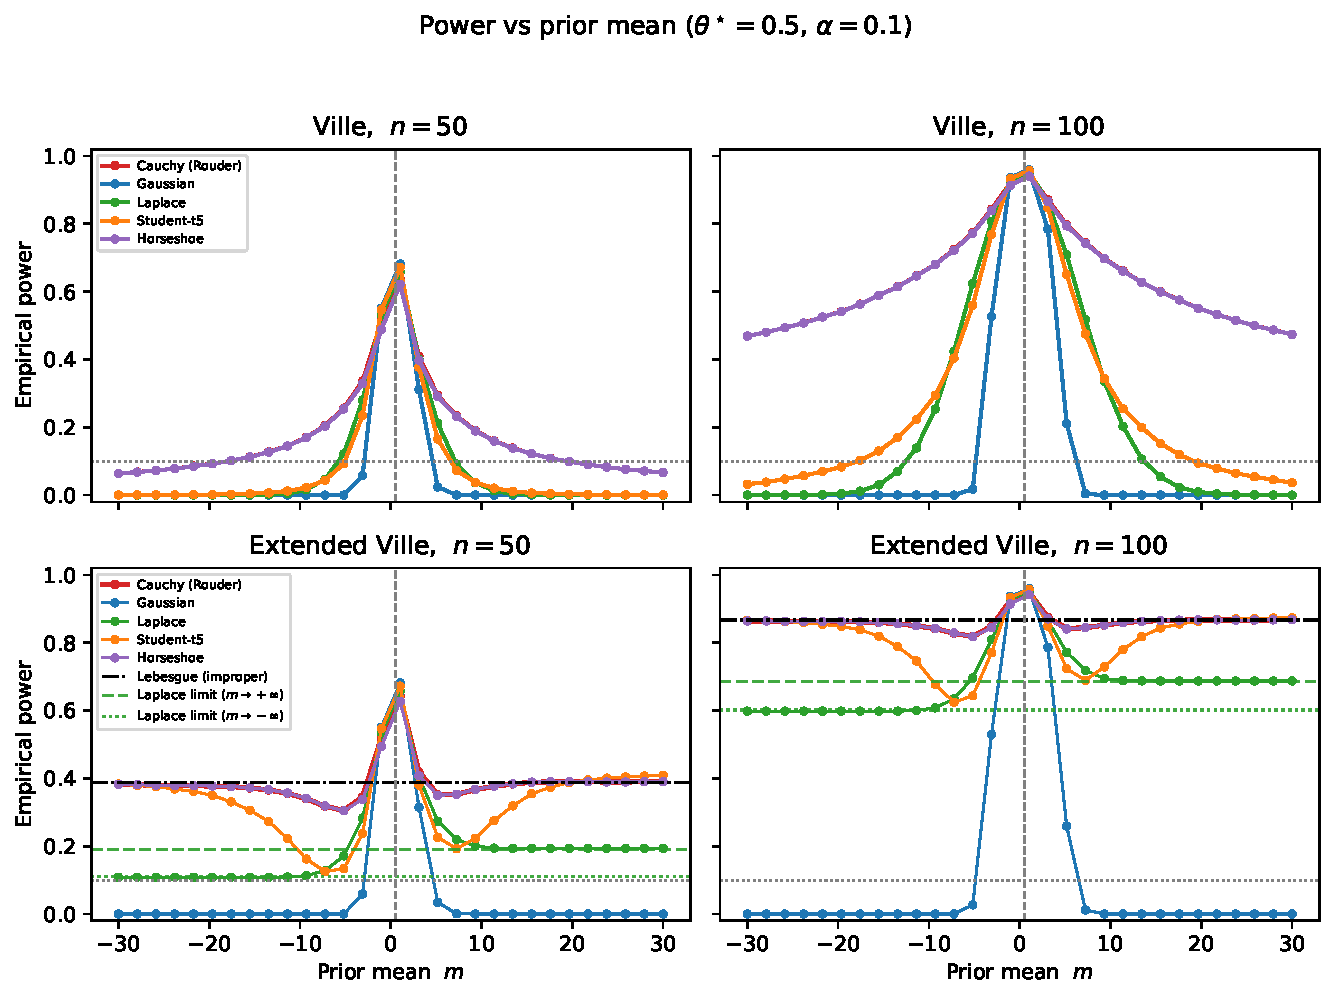
\includegraphics[width=0.7\textwidth]{images/power_vs_m_priors_poster.pdf}
    \end{figure}

    \vspace{-0.15cm}
    {\small
    % Empirical power as a function of prior location $|m|$ under $\theta^{\star}=0.5$, $\alpha=0.1$, sample size $n\in\{5,20,50,100,200\}$.

    % \textbf{Colour key.}
    % \textcolor{red!70!black}{\textbf{Cauchy}} (polynomial, $\beta=2$),
    % \textcolor{orange!90!black}{\textbf{Student-$t_5$}} (polynomial),
    % \textcolor{purple}{\textbf{horseshoe}} (polynomial),
    % \textcolor{green!55!black}{\textbf{Laplace}} (exponential),
    % \textcolor{blue}{\textbf{Gaussian}} (sub-Gaussian),
    % \textcolor{gray}{\textbf{Lebesgue baseline}} (dash-dotted).

    \textbf{Top -- classical Ville.} Every proper prior is fragile under conflict: power collapses to zero as $|m|$ grows. This is precisely the failure mode that motivates the extended Ville calibration.

    \textbf{Bottom -- extended Ville.} \textcolor{orange}{\textbf{Polynomial}}-tail priors gain power under prior-data agreement and \emph{gracefully revert to the Lebesgue baseline} (dash-dotted) under conflict, confirming Theorem 6. The \textcolor{blue}{\textbf{Gaussian}} curve collapses (Theorem 8); \textcolor{DeepGreen}{\textbf{Laplace}} plateaus at the tilted limit (Theorem 4).
    }
  \end{block}

\begin{block}{References}
\bibliographystyle{alpha}
\footnotesize{
\bibliography{bayesanytimettest.bib}}
\end{block}



  % \begin{block}{References}
  %   \footnotesize
  %   \begin{itemize}
  %     \setlength\itemsep{0.05cm}
  %     \item Cortinovis, Kilian, Caron (2025). Anytime-valid $t$-tests with informative priors.
  %     \item Lai (1976). On confidence sequences. \emph{Ann.\ Statist.}
  %     \item P\'erez-Ortiz, Lardy, de Heide, Gr\"unwald (2024). E-statistics, group invariance and anytime-valid testing.
  %     \item Rouder, Speckman, Sun, Morey, Iverson (2009). Bayesian $t$-tests for accepting and rejecting the null. \emph{Psychon.\ Bull.\ Rev.}
  %     \item Wang, Ramdas (2025a). Anytime-valid $t$-tests for Gaussian means with unknown variance.
  %     \item Wang, Ramdas (2025b). The extended Ville's inequality.
  %   \end{itemize}
  % \end{block}

\end{column}

\separatorcolumn
\end{columns}
\end{frame}
\end{document}